% DO NOT COMPILE THIS FILE DIRECTLY!
% This is included by the other .tex files.

\begin{frame}
\titlepage
\end{frame}


\section{What has happened since the last MUG}

\section{Give you a brief update over the highlights}

\begin{frame}
  \frametitle{A Topical Listing of the New Major Features}
  \begin{itemize}
      \item Improved data model in MISP to support \textbf{analyst data} including analyst notes, opinions, and relationships
      \item \textbf{Workflow} improvements and changes to support use-cases
      \item \textbf{STIX 2.1} improvements along with MISP galaxy 2.0 support
      \item Performance improvements including in the MISP sighting, synchronization, and ReST queries
      \item \textbf{Logging/Monitoring} and \textbf{security} improvements
      \item \textbf{MISP modules} are now autonomous
      \item \textbf{Security fixes} and other improvements
  \end{itemize}
\end{frame}

\begin{frame}
  \frametitle{Analyst Data}
  \begin{itemize}
       \item The Analyst Data feature\footnote{Extending the MISP standard format} is an extended and shareable set of capabilities that allows analysts \textbf{to share and add their own analysis to any MISP event}.
       \item The Analyst Data feature comprises three main components:
       \begin{itemize}
             \item Adding an \textbf{Analyst Note} to any element in MISP, such as Event, Event Report, Object, Attribute, or Galaxy Cluster.
             \item Adding an \textbf{Analyst Opinion} with a rating (between 0 and 100) to any element in MISP, such as Event, Event Report, Object, Attribute, Galaxy Cluster, or Analyst Note.
             \item Adding an \textbf{Analyst Relationship} from/to any element in MISP with a specified relationship type.
       \end{itemize}
  \end{itemize}
\end{frame}

\begin{frame}
   \frametitle{Analyst Opinion and Note View}
   \begin{itemize}
        \item Showing/editing opinion on a MISP event or a MISP galaxy cluster
   \end{itemize}
   \begin{center}
        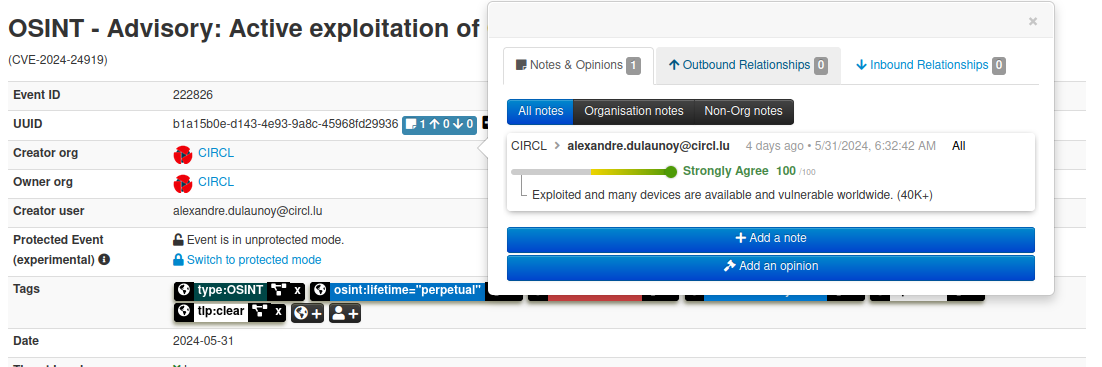
\includegraphics[scale=0.2]{opinion.png}
        \hspace{1cm}
        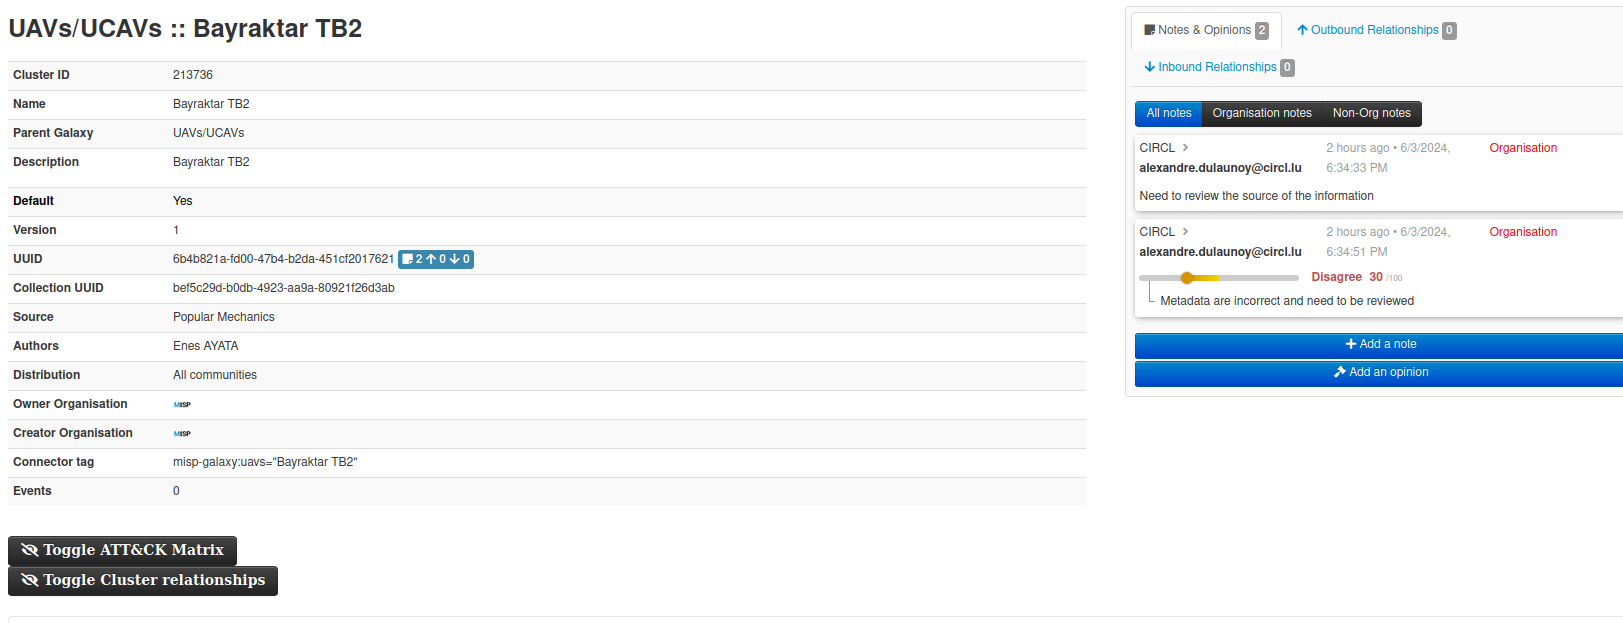
\includegraphics[scale=0.19]{note.png}
   \end{center}
\end{frame}

\begin{frame}
	\frametitle{Analyst Relationship}
	\begin{itemize}
	          \item Showing/editing a relationship between a MISP galaxy cluster and another element
	\end{itemize}
	\begin{center}
	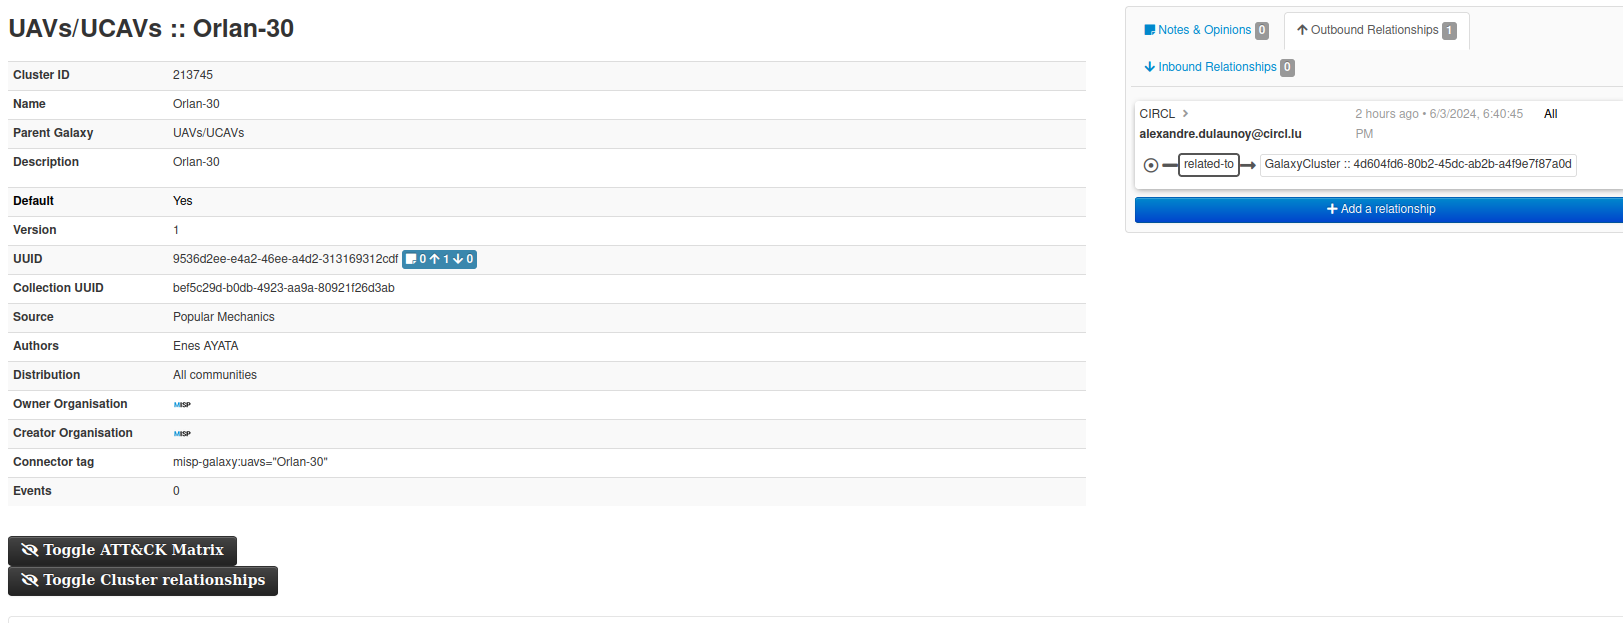
\includegraphics[scale=0.2]{relationship.png}
	\end{center}
\end{frame}

\begin{frame}
  \frametitle{Workflows}
  \begin{itemize}
     \item Additional \textbf{action nodes} like Slack added as action module in MISP modules
     \item Inclusion of new \textbf{triggers} based on community feedback
     \item Distribution-if module now includes sharing-group
     \item Various workflow bugs fixed following community feedback
  \end{itemize}
\end{frame}

\begin{frame}
\frametitle{Workflows}
\begin{center}
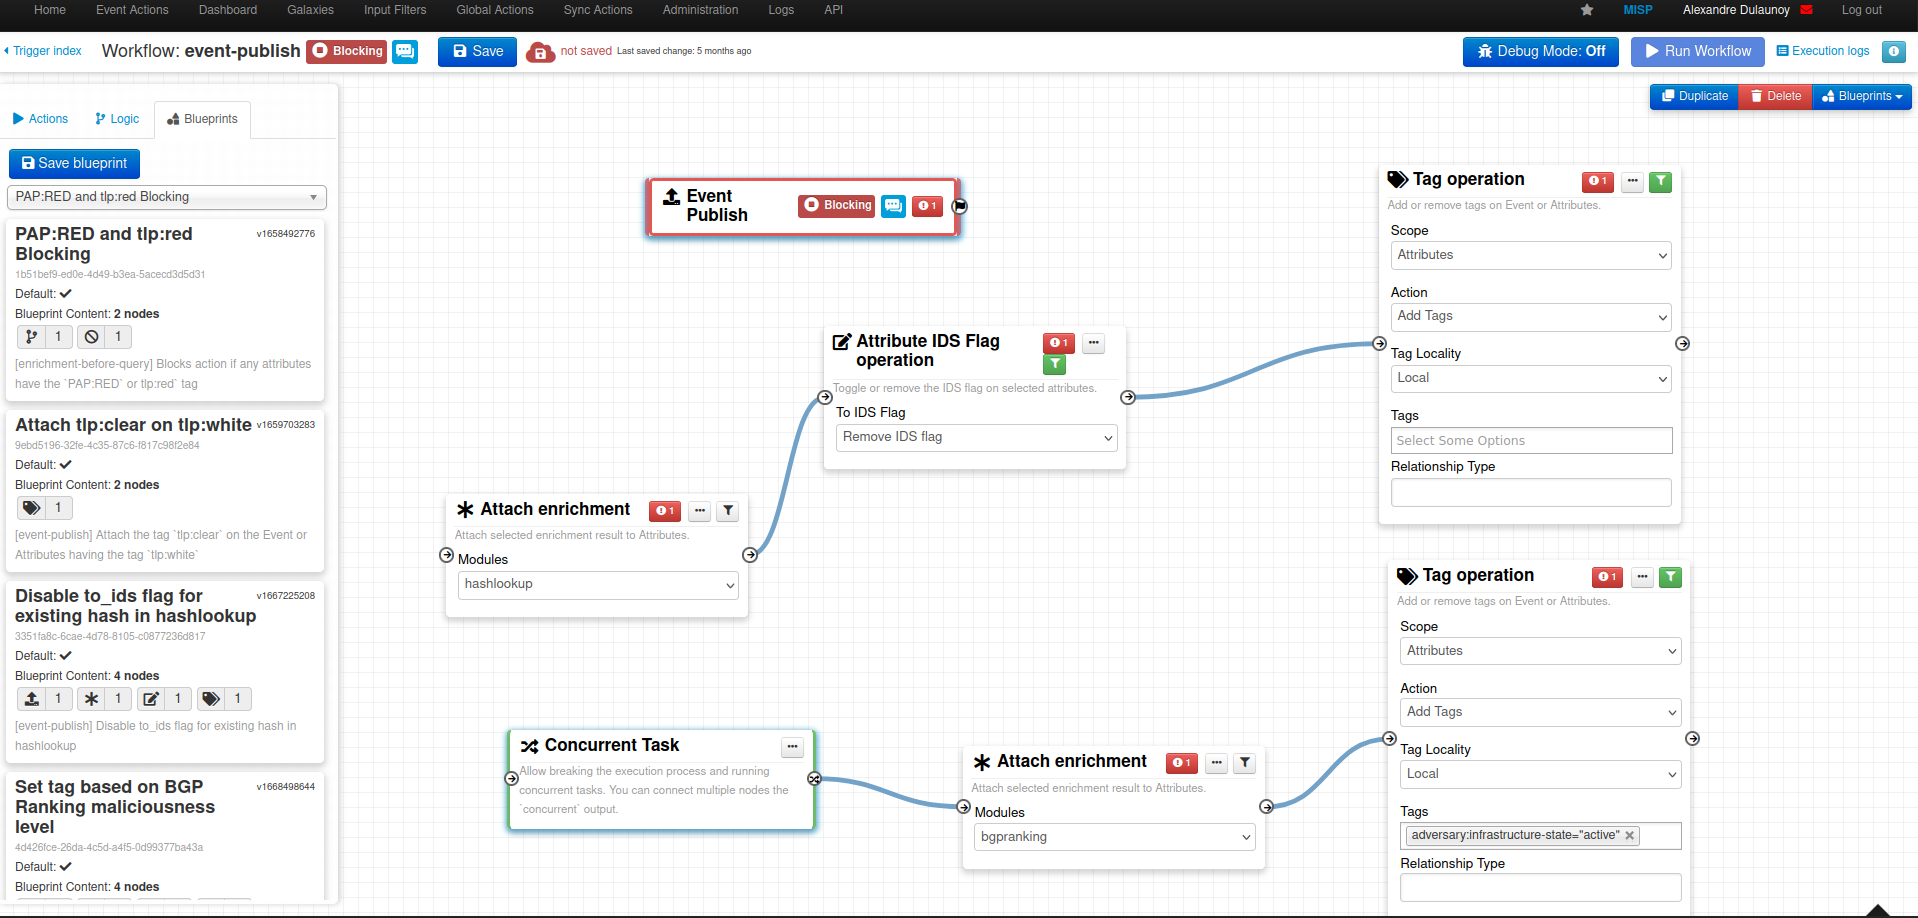
\includegraphics[scale=0.17]{images/workflows_filtered.png}
\end{center}
\end{frame}

\begin{frame}
  \frametitle{Performance and Sightings}
  \begin{itemize}
     \item Fast API authentication allowing the storage of hashed API keys in Redis (optional)
     \item Option to disable the loading of sightings via the API
     \item Support for a sighting policy (\texttt{getLastSighting}) and blocking sighting sync per organisation
     \item Attribute fetch refactored to simplify conditions and limit the loading of ACL
     \item Attribute search reworked for performance improvement
     \item New benchmarking suite added, collecting metrics, all accessible in the dashboard widget
  \end{itemize}
\end{frame}

\begin{frame}
  \frametitle{Security Fixes and Other Improvements}
  \begin{itemize}
     \item Long list of security fixes based on multiple external penetration tests
     \item \textbf{CVEs}\footnote{\url{https://www.misp-project.org/security/}} continuously reported for issues small and large
     \begin{itemize}
         \item Make sure you're up to date and have TOTP active on your MISP instance.
     \end{itemize}
     \item Research by \textbf{Zigrin Security}, funded by the \textbf{Luxembourg Army}, has been a massive help along with recent pentests from NATO
     \item Long list of other improvements, quality of life changes, and performance tuning
  \end{itemize}
\end{frame}


\begin{frame}
\frametitle{MISP Modules}
    \begin{itemize}
        \item MISP modules\footnote{\url{https://github.com/MISP/misp-modules/}} are companions for expansion, export, and import for external services or tooling
	\item New modules added, such as the {\bf Google Threat Intelligence expansion module}
        \item New workflow action modules added, such as Slack, with improvements to the Mattermost module
        \item Many improvements and fixes to all the modules
    \end{itemize}
\end{frame}

\begin{frame}
\frametitle{MISP Modules are Now Standalone}
    \begin{itemize}
        \item MISP Modules\footnote{\url{https://www.misp-project.org/2024/03/12/Introducing.standalone.MISP.modules.html/}} can now function independently of the MISP platform.
        \item A versatile web interface is now available where you can query different modules, keep a history, and facilitate pivoting.
    \end{itemize}
    \begin{center}
        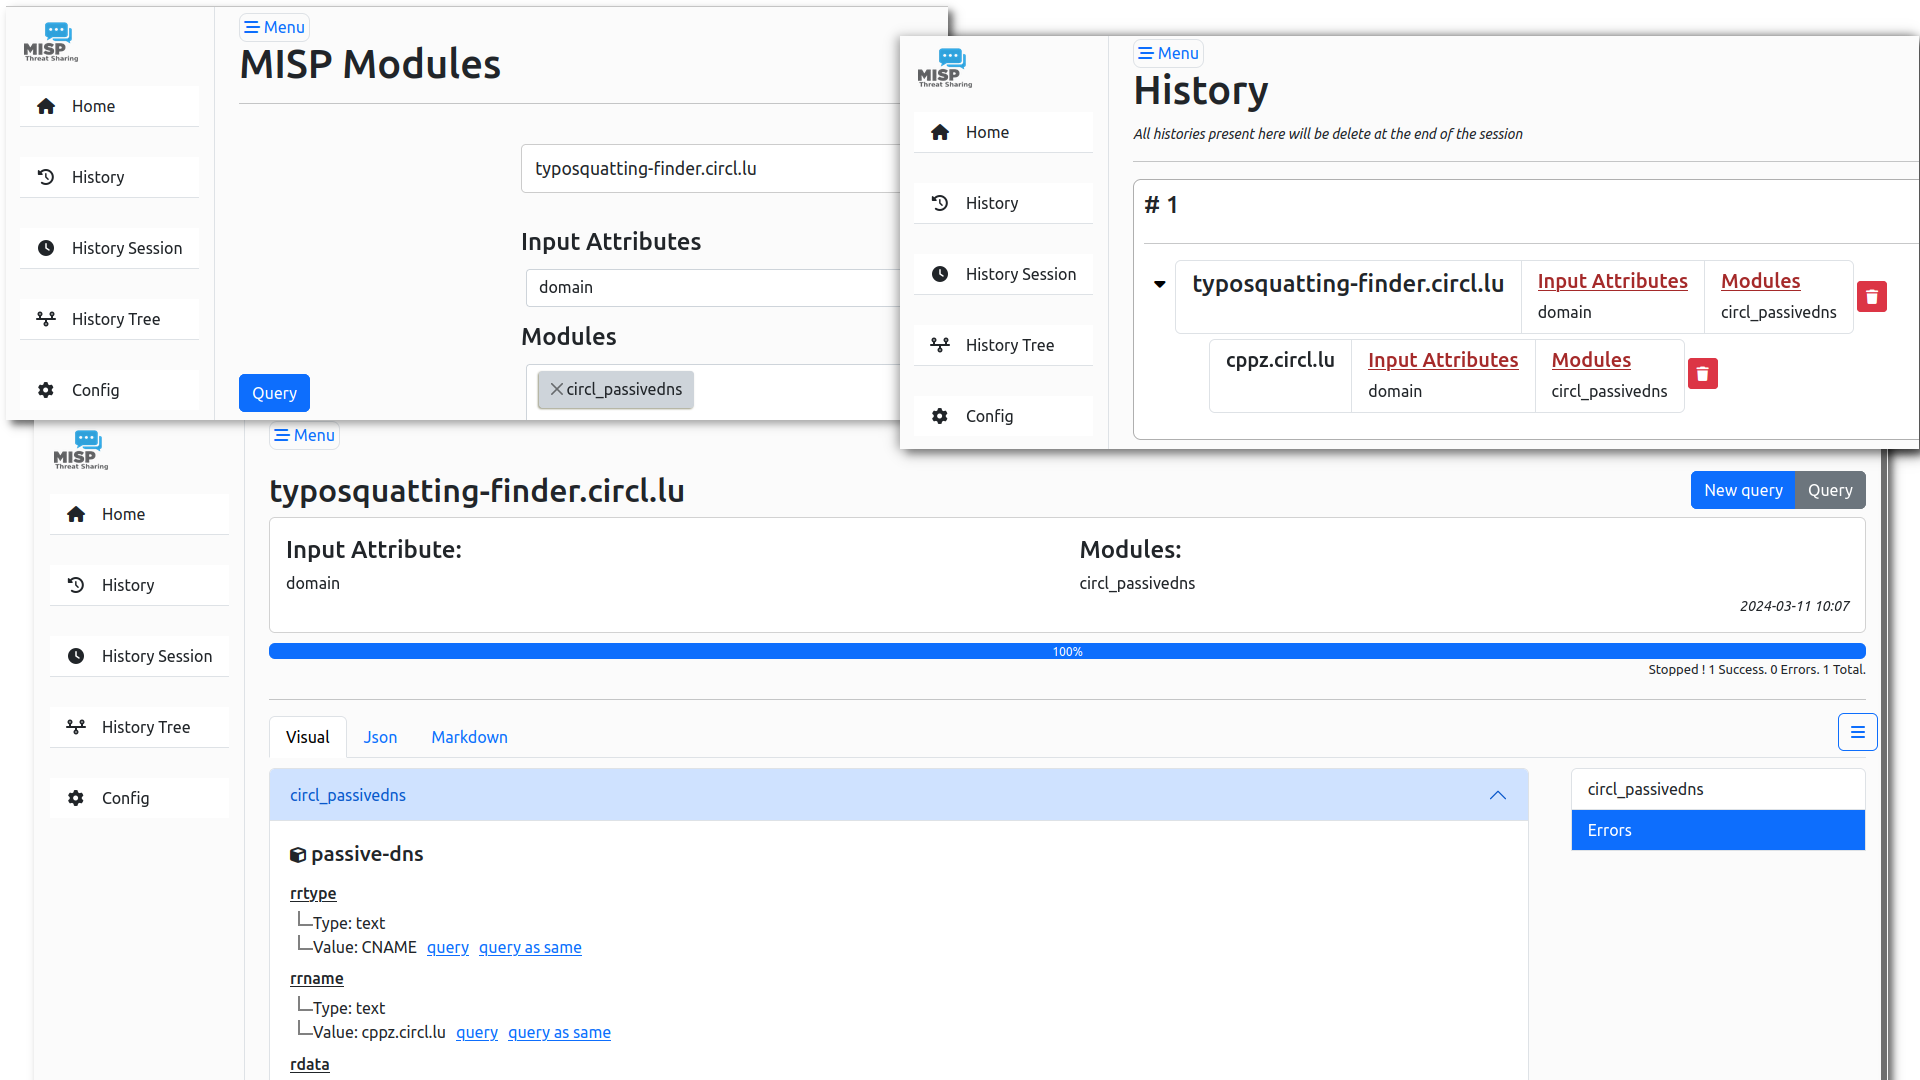
\includegraphics[scale=0.5]{all-modules.png}
    \end{center}
\end{frame}

\begin{frame}
    \frametitle{MISP Taxonomies}
    \begin{itemize}
        \item 149 ready-to-use taxonomies are now available in MISP\footnote{\url{https://github.com/MISP/misp-taxonomies/}} (used in MISP and many other tools)
        \item Improved \textbf{dark-web} taxonomy to map the use of JRC with the AIL project\footnote{\url{https://www.ail-project.org/}}
        \item Many improvements to the different taxonomies including \textbf{workflow}, \textbf{event-type}, and many others
    \end{itemize}
\end{frame}

\begin{frame}
    \frametitle{MISP Warning-Lists}
    \begin{itemize}
        \item New \textbf{check-host.net} warning-list added
        \item New \textbf{link-in-bio} warning-list added (similar to URL shortener)
        \item New \textbf{find-ip} known hostname used for querying your source IP (collected from our Passive DNS)
        \item Many updates in the existing warning-lists such as the \textbf{URL shortener}
    \end{itemize}
\end{frame}

\begin{frame}
    \frametitle{MISP galaxy}
    \begin{itemize}
	\item New website for MISP galaxy\footnote{\url{https://www.misp-galaxy.org/}} is now online including inter-relationship between galaxies
	\item Latest MITRE ATT\&CK version 15.1 updated for the MISP galaxy
        \item New {\bf producer} galaxy to facilitate the link to security reports with their respective producers
	\item New {\bf INTERPOL Dark Web and Virtual Assets Taxonomies}, {\bf UKHSA Culture Collections}, {\bf Threat Matrix for Storage Services}, {\bf Intel Agencies}, {\bf Tidal}
	\item Major updates in {\bf Disarm}, {\bf threat-actor}, {\bf Surveillance Vendor} and {bf ransomware} galaxies
    \end{itemize}
\end{frame}

\begin{frame}
    \frametitle{Matrix-based MISP galaxy}
    \begin{center}
	    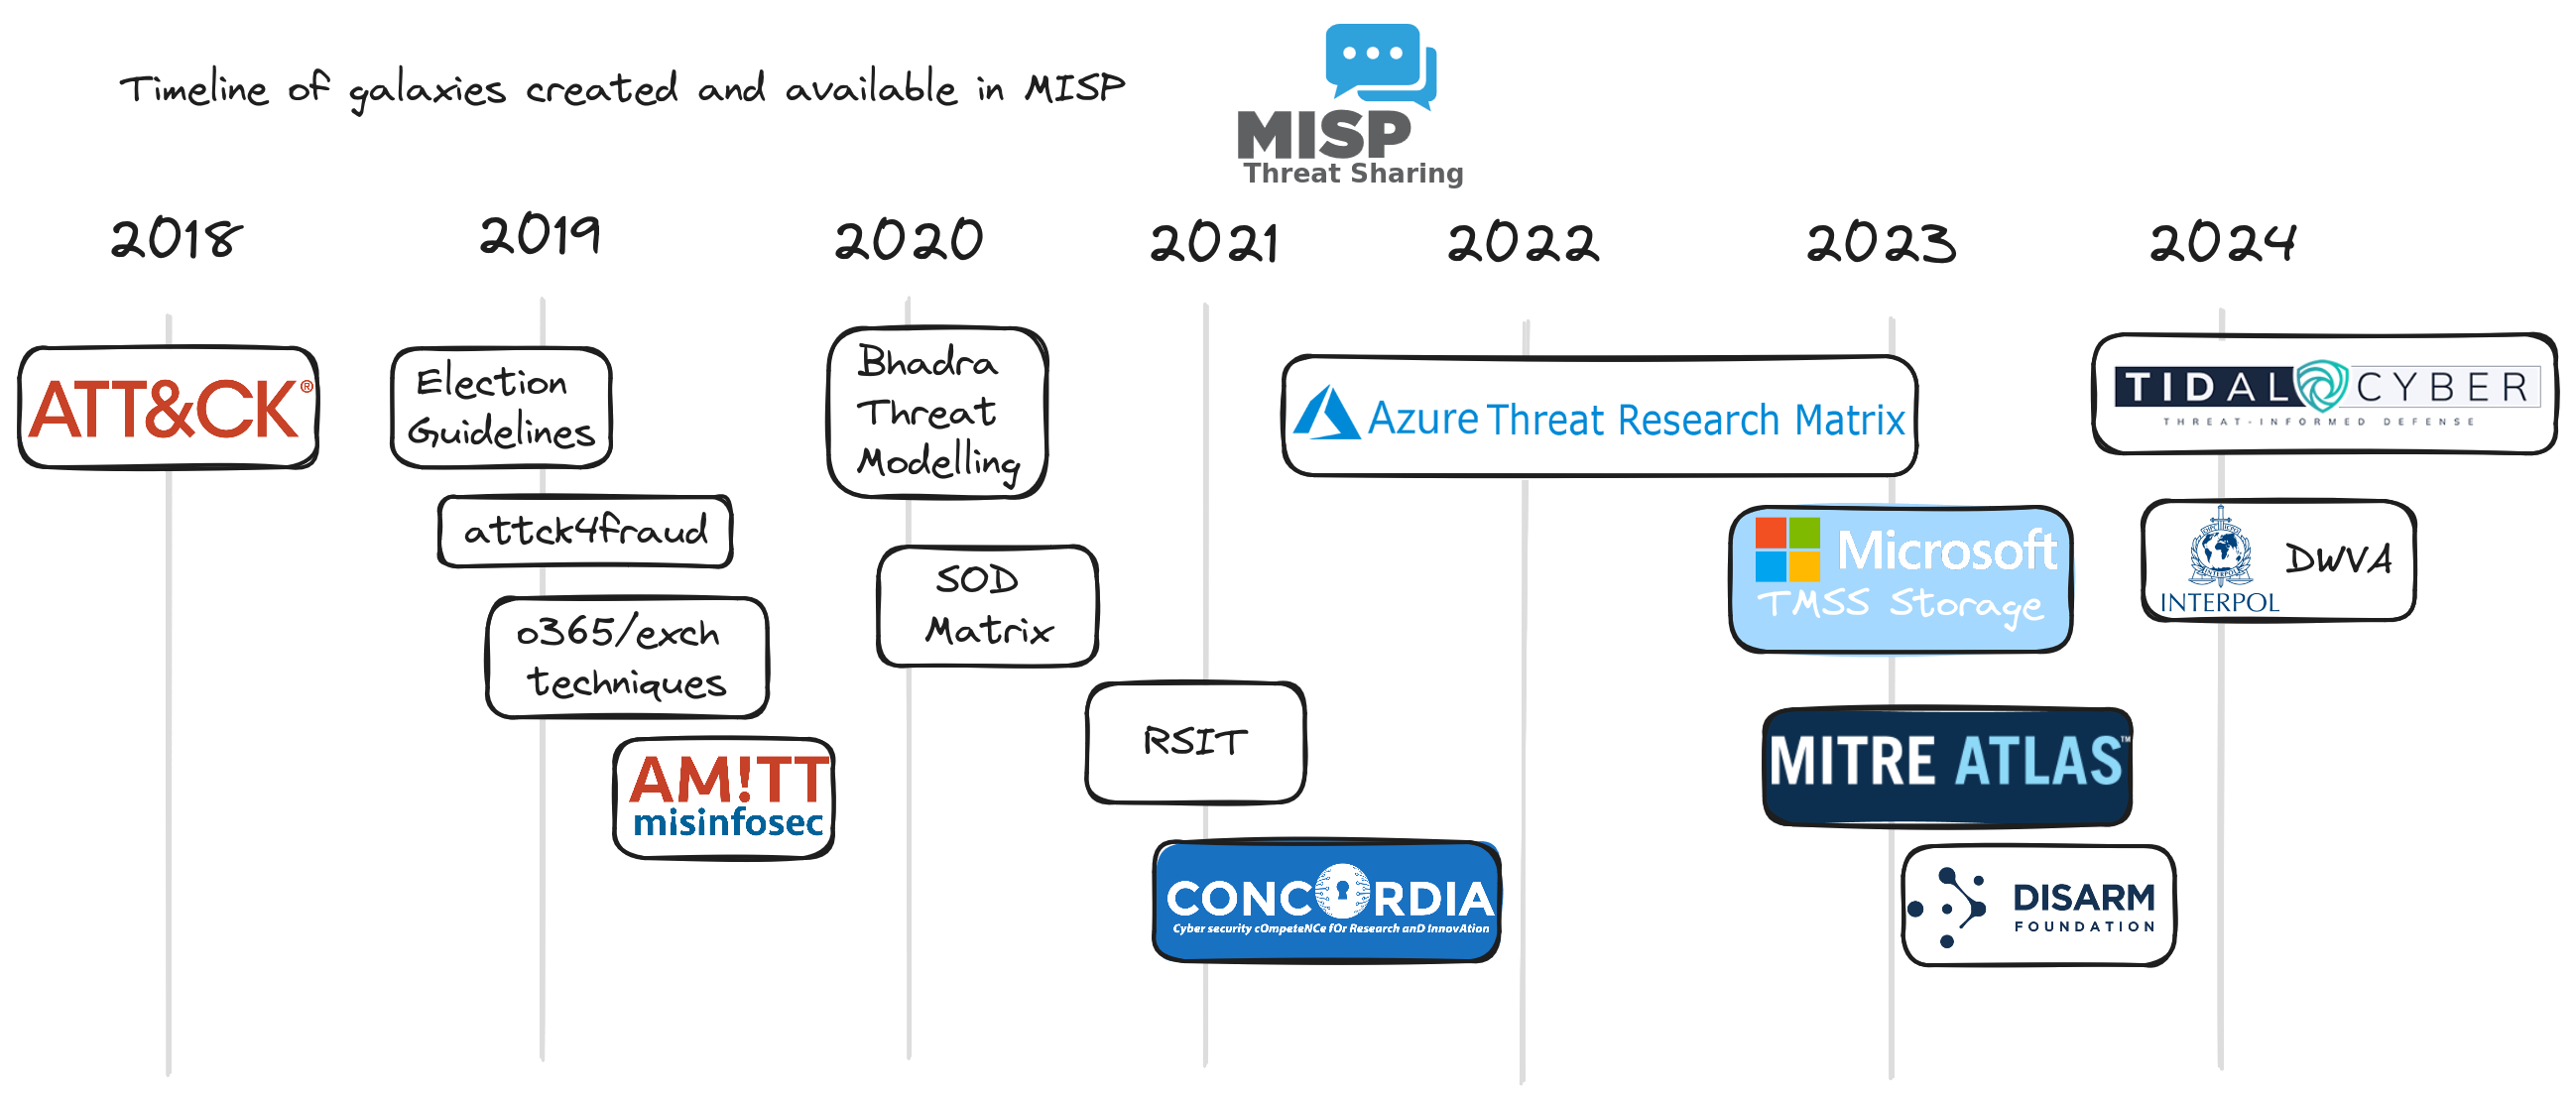
\includegraphics[scale=0.14]{timeline.png}
    \end{center}
\end{frame}

\begin{frame}
    \frametitle{MISP Objects}
    \begin{itemize} 
        \item Improvement in \textbf{cs-beacon-config} to map Shadow Server discovery service of CS
        \item Improvement of \textbf{ransomware-group-post} to map other discovery services such as ransomlook.io
        \item New objects to support Flowintel\footnote{\url{https://github.com/flowintel/flowintel-cm}} cases and tasks
        \item New object \textbf{generalizing-persuasion-framework} requested for disinformation use-cases
        \item Many improvements to existing objects, including fixes for STIX 2.1 or CERT.PL use-cases
        \item Many new default relationships added to the MISP objects
    \end{itemize}
\end{frame}

\begin{frame}
     \frametitle{MISP stix}
     \begin{itemize}
        \item misp-stix\footnote{\url{https://github.com/MISP/misp-stix}} is standalone Python library support MISP standard format and all the STIX version (1.1.1, 1.2, 2.0 and 2.1)
        \item Two people from CIRCL are {\bf co-sharing the OASIS Cyber Threat Intelligence (CTI) TC and CTI STIX subcommittee}
        \item Ensuring alignment between the standards, interoperability and an open source standard library
     \end{itemize}
\end{frame}

\begin{frame}
     \frametitle{MISP stix - Custom Galaxy Cluster Import}
     \begin{itemize}
	\item TTPs, Threat Actors and other contextual descriptions imported as Galaxy Clusters
	\item Generating specific Custom Galaxy Clusters from STIX directly
     \end{itemize}
     \begin{center}
	  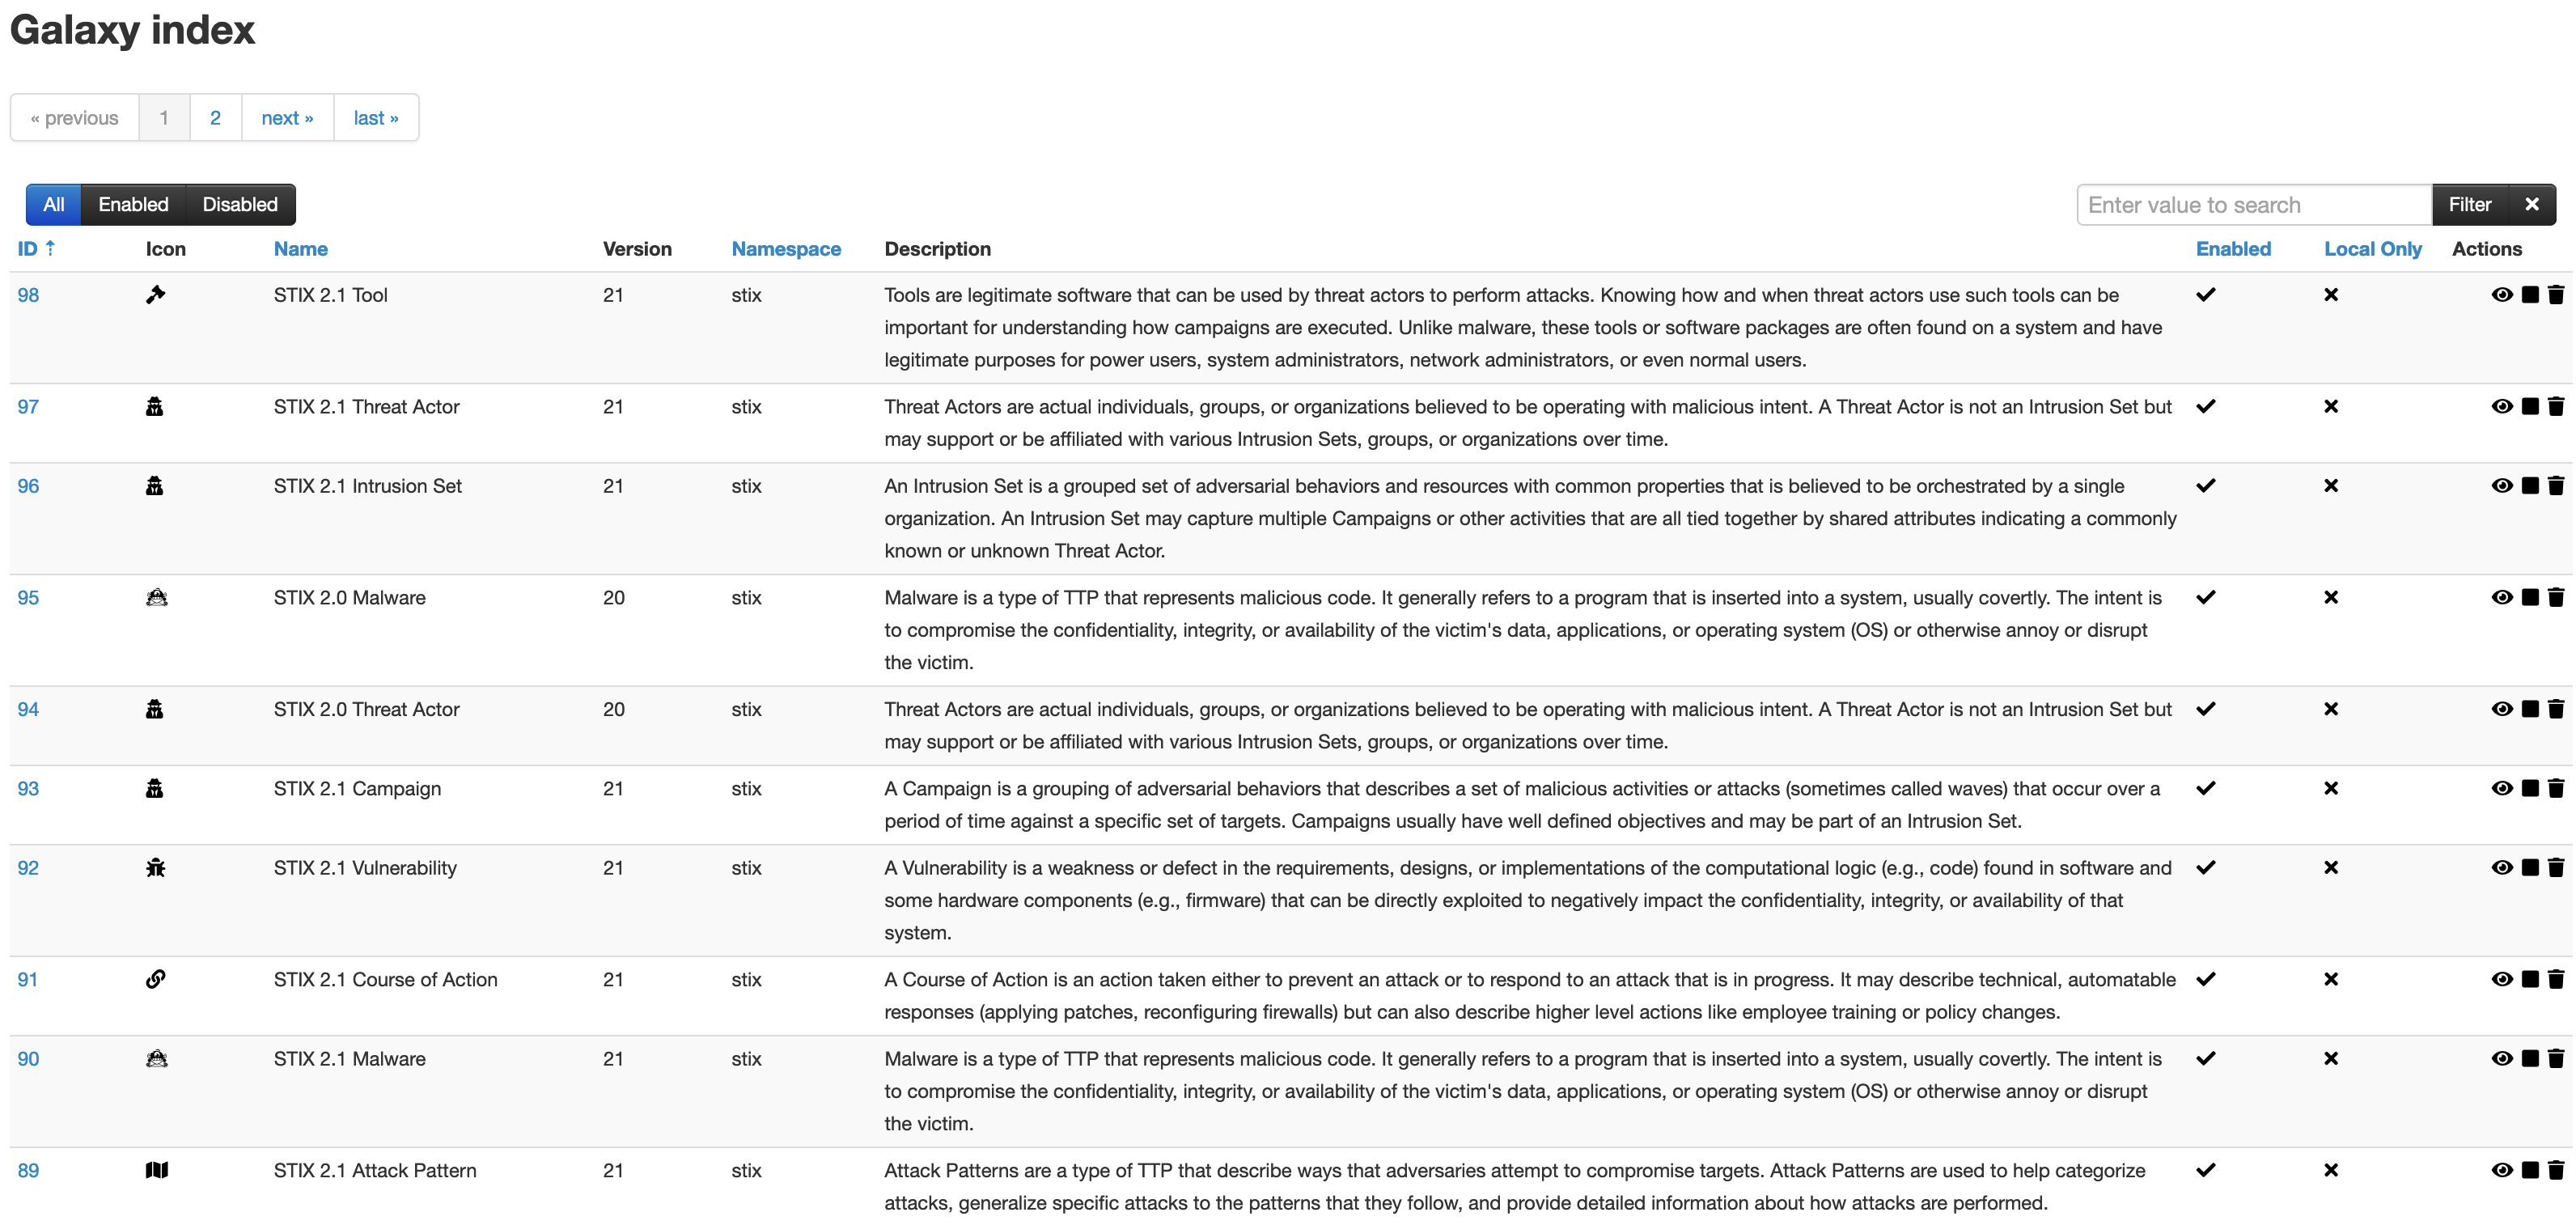
\includegraphics[scale=0.1]{stix-cluster.png}
	  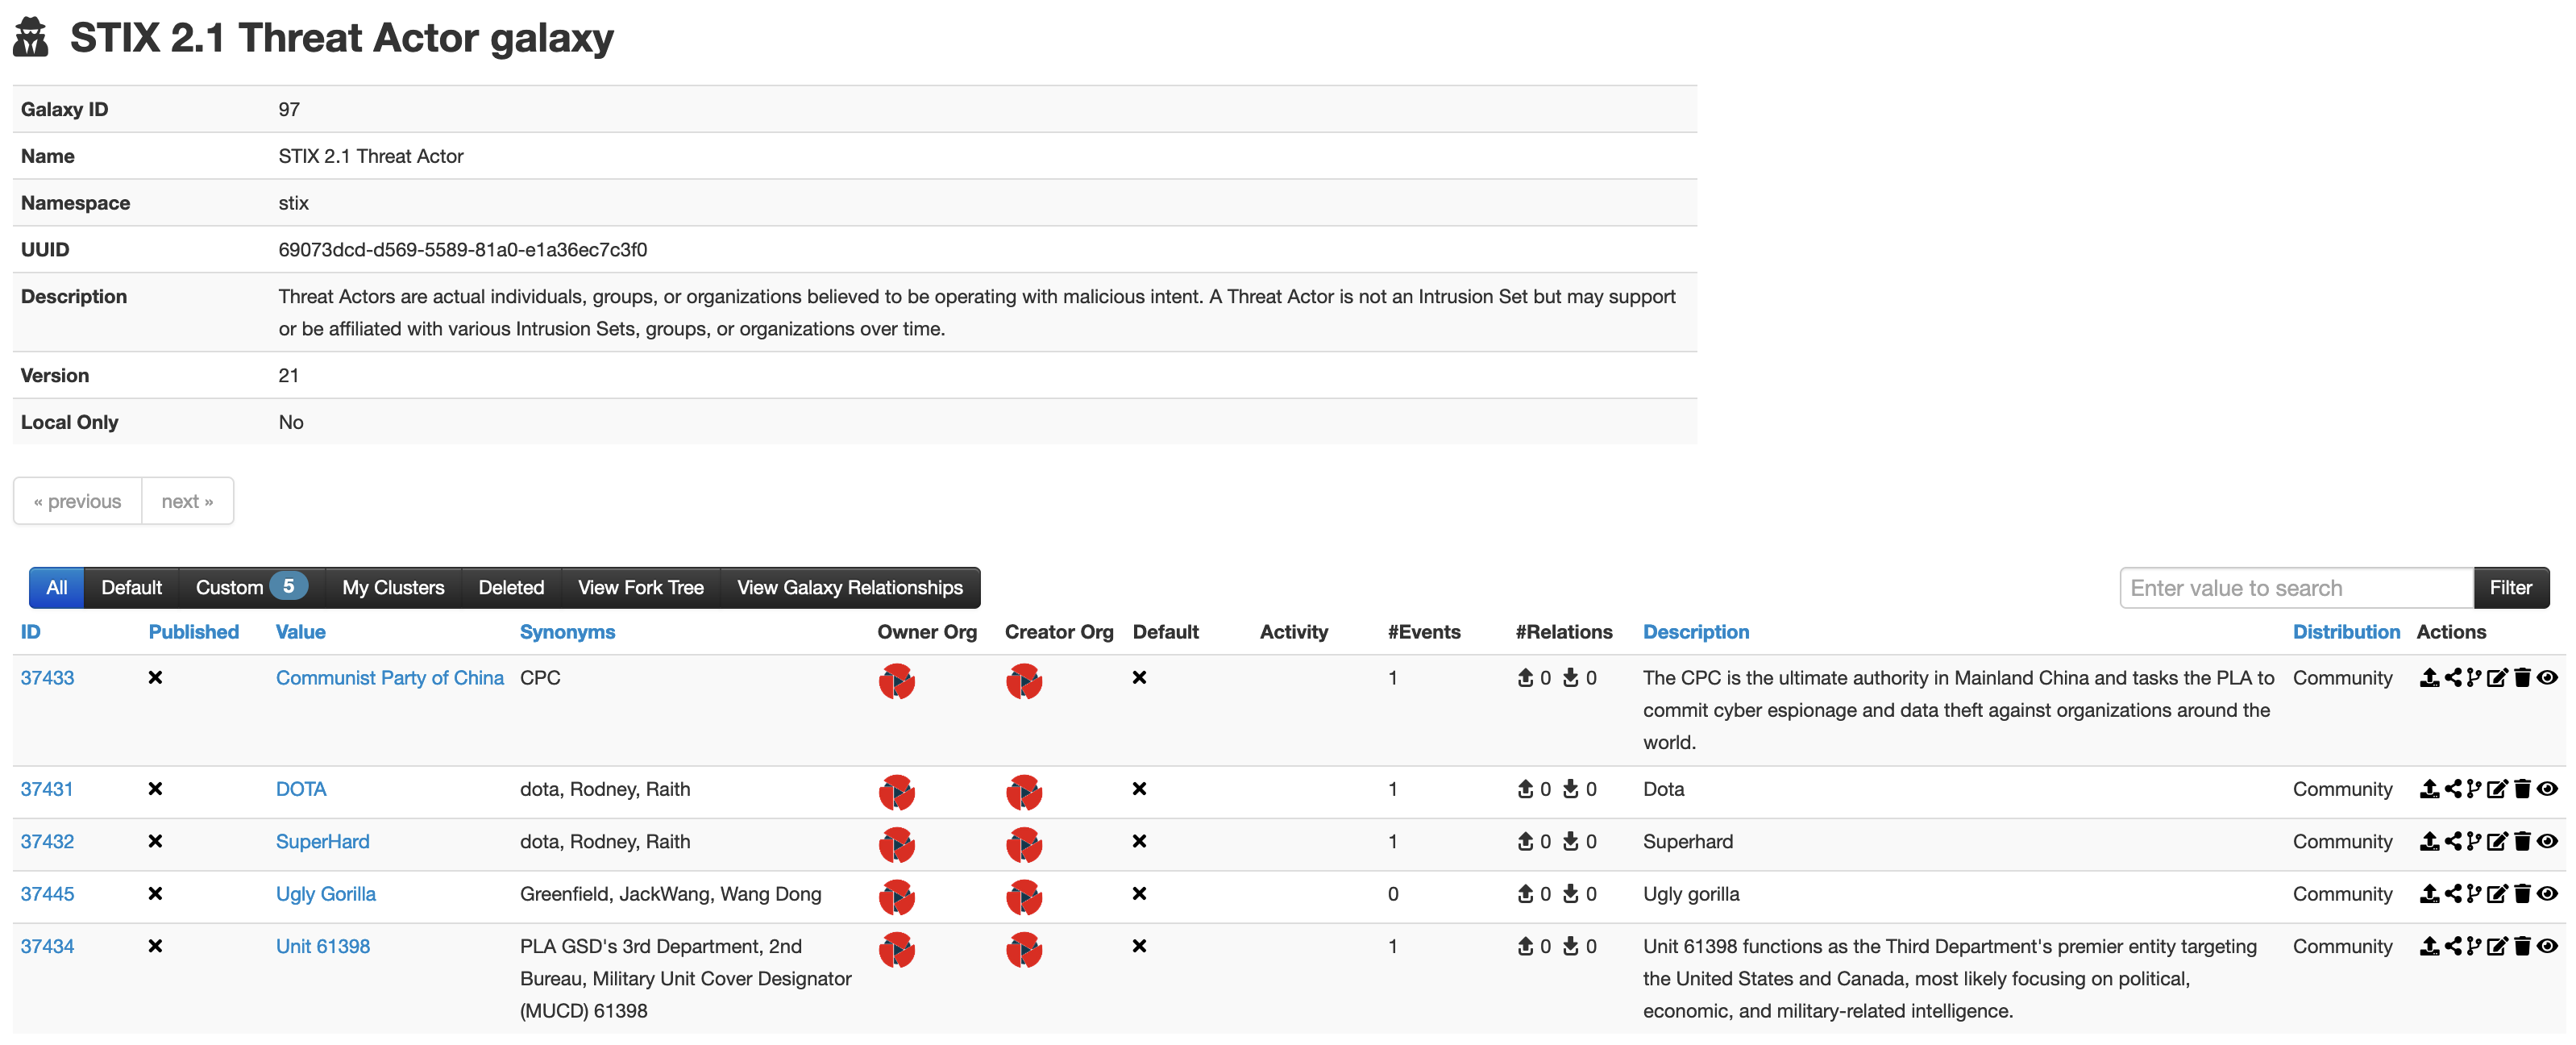
\includegraphics[scale=0.1]{stix-cluster2.png}
     \end{center}
\end{frame}

\begin{frame}
     \frametitle{MISP stix - Custom Galaxy Cluster Import}
     \begin{itemize}
        \item Extracting the complete description within the Cluster meta fields
	\begin{center}
	   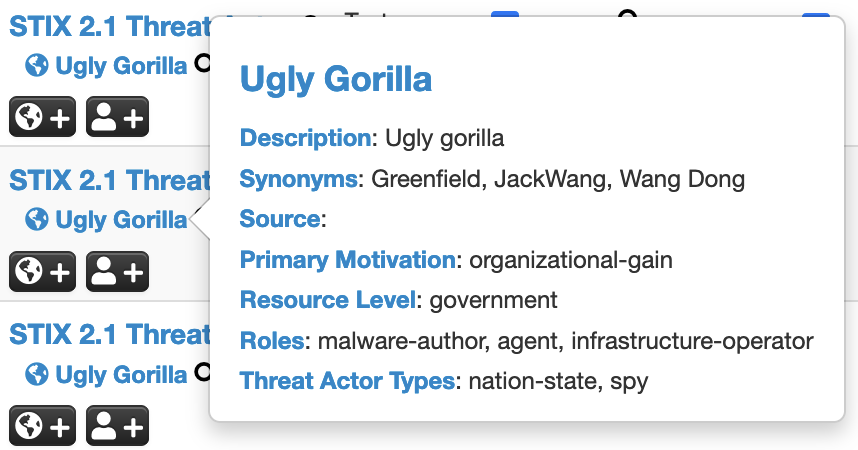
\includegraphics[scale=0.5]{stix-cluster3.png}
        \end{center}
     \end{itemize}
\end{frame}

\begin{frame}
     \frametitle{MISP stix - Distribution and MISP Galaxy 2.0}
     \begin{itemize}
        \item Ability to select the Clusters distribution
     \end{itemize}
	\begin{center}
	    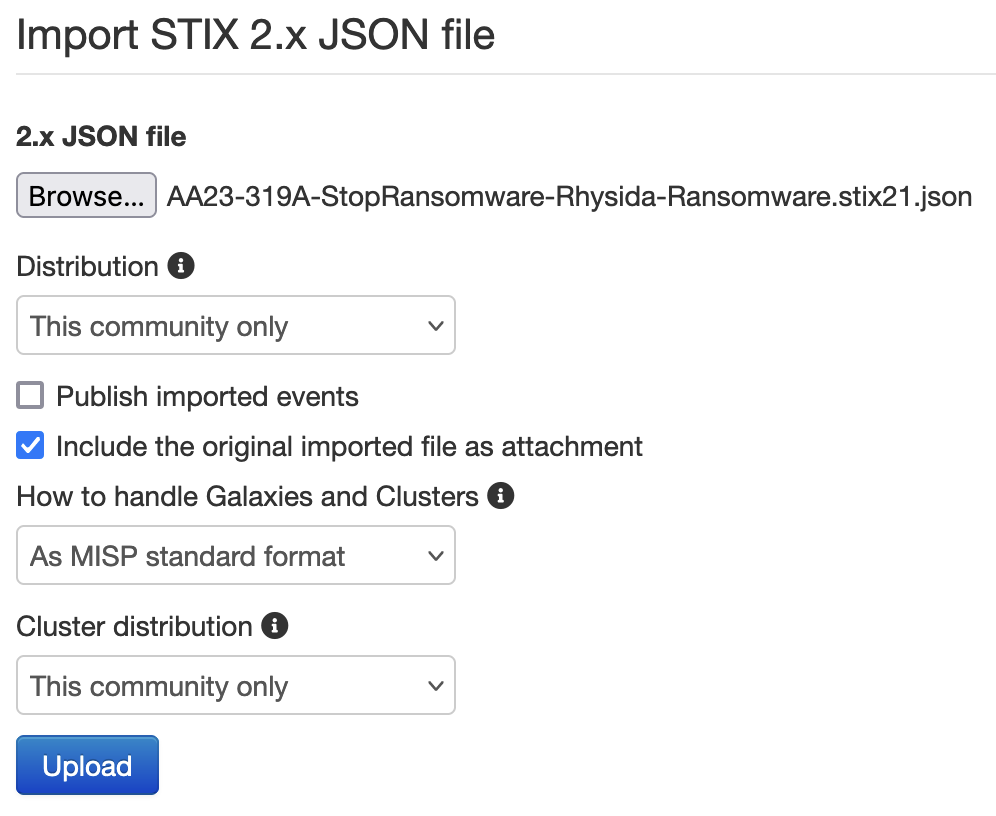
\includegraphics[scale=0.5]{stix-cluster4.png}
	\end{center}
\end{frame}

\begin{frame}
     \frametitle{MISP stix - Support of ACS markings}
     \begin{itemize}
	     \item Generating a {\bf Custom Galaxy Cluster} with the flattened description of the the Marking definition
             \item Extracting some of the fields as Tag to provide classification of the data marked with the Marking definition
     \end{itemize}
	\begin{center}
	    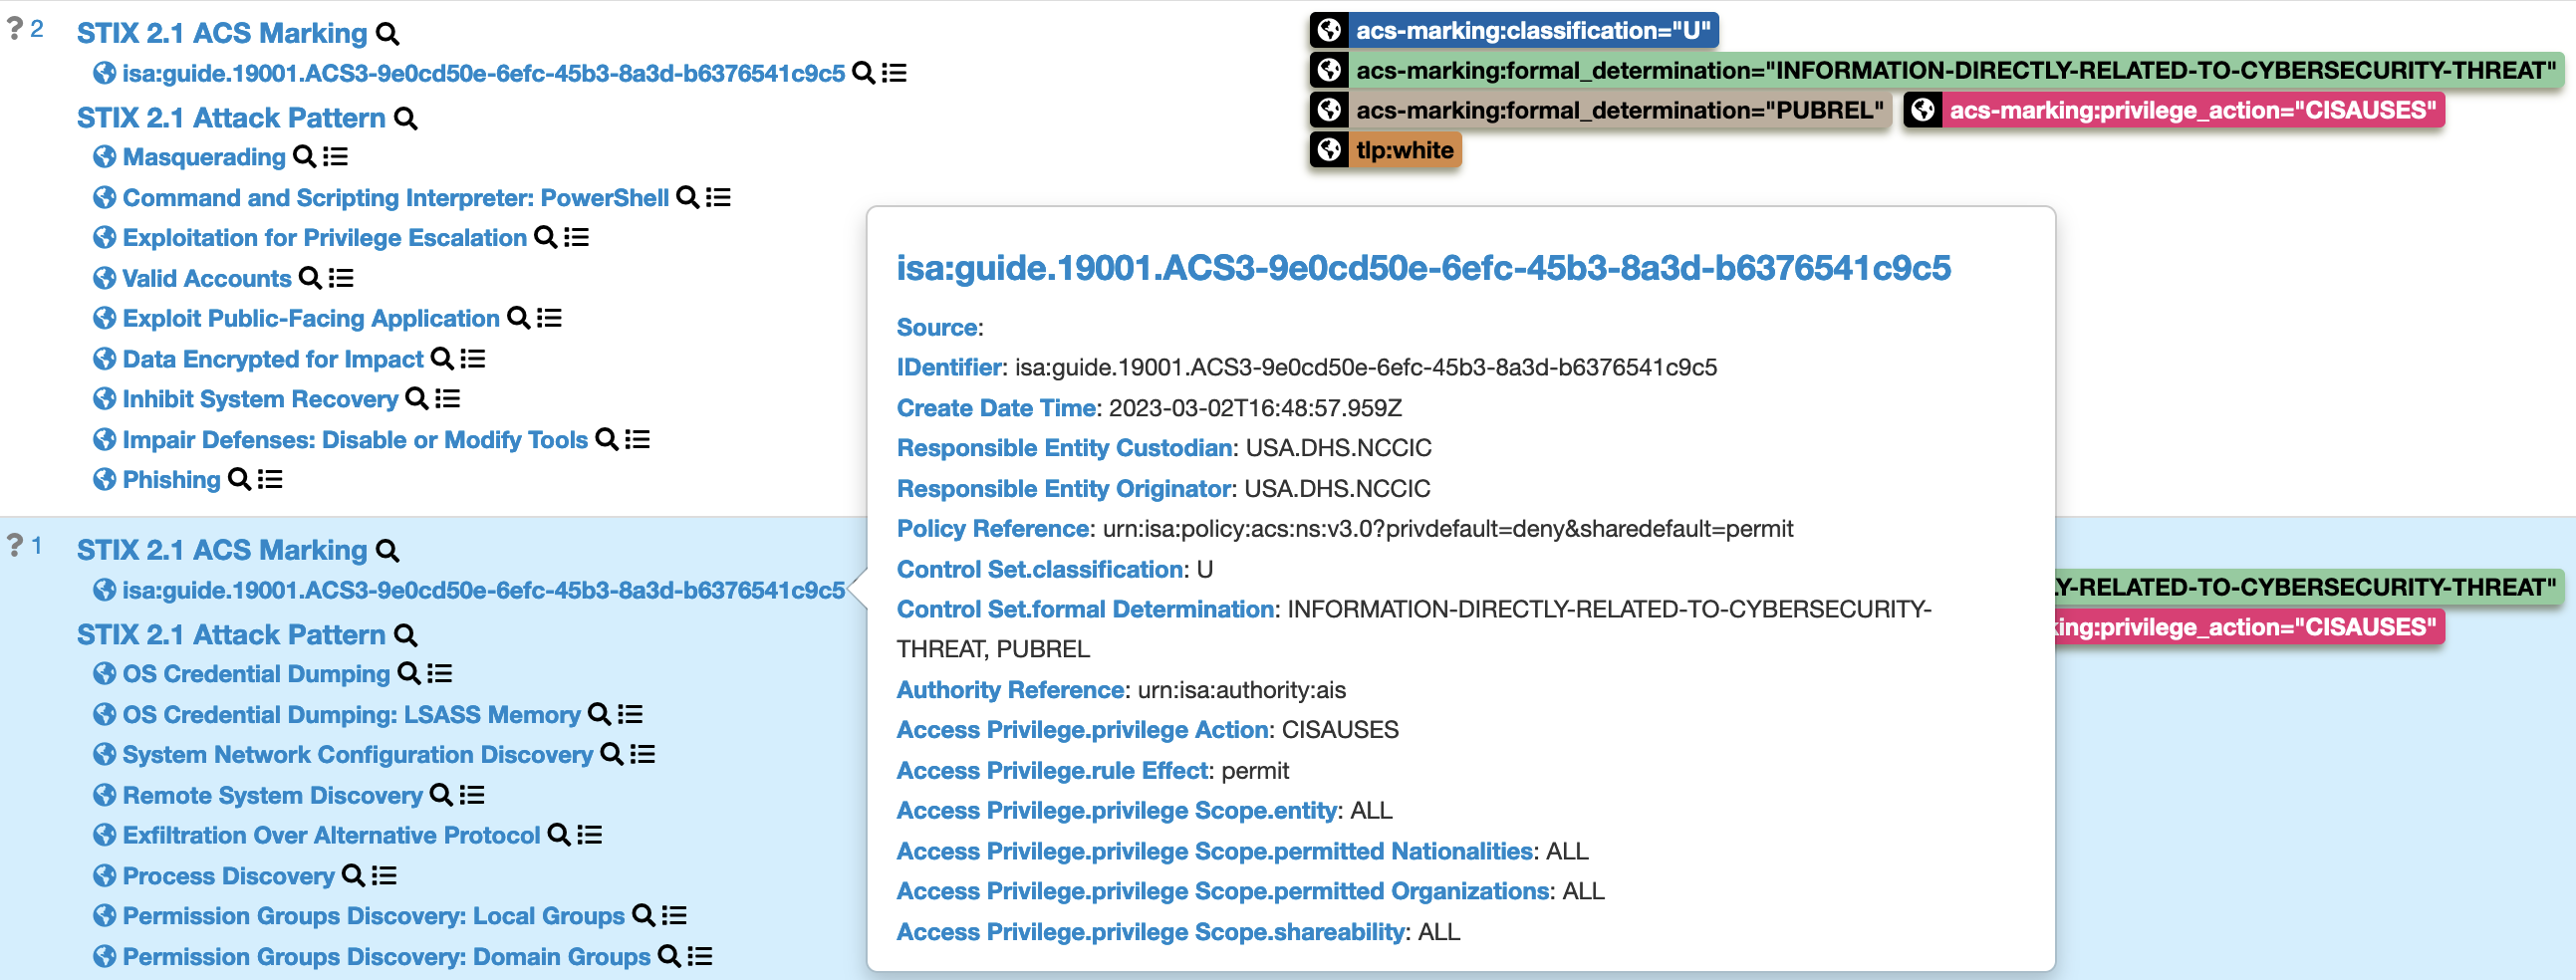
\includegraphics[scale=0.4]{stix-cluster5.png}
        \end{center}
\end{frame}

\begin{frame}
       \frametitle{Continuous improvement \& Work in progress}
	\begin{itemize}
		\item Import {\bf Note \& Opinion} objects using the recently released {\bf Analyst Data} feature
		\item Filling the mapping gaps between {\bf Indicators, Observed Data, Observable objects} and their MISP representation ({\bf Attributes \& Objects})
	\end{itemize}
\end{frame}

\begin{frame}
    \frametitle{Cerebrate}
    \begin{itemize}
        \item Cerebrate v1.19\footnote{\url{https://www.cerebrate-project.org/2024/05/15/Cerebrate-version-1.19-released.html}} released with several usability and functionality fixes (v1.20 is expected this week)
        \item Many \textbf{improvements and bugs fixed} following feedback from various organizations deploying Cerebrate, such as the ENISA CSIRT network
        \item Deployment of the \textbf{PoC for NATO users is ongoing} - Cerebrate instance will be available on 15th September 2024
    \end{itemize}
\end{frame}

\section{Ongoing rework}

\begin{frame}
  \frametitle{MISP 3}
  \begin{itemize}
     \item Largest ongoing work is the work on {\bf MISP3}
     \item Already announced long ago, development is now underway\footnote{\url{https://github.com/MISP/MISP/tree/3.x}}
     \item New {\bf tech stack} based on Cerebrate's advances (CakePHP 4.x+, PHP 8.2+, Bootstrap 5+)
     \item Longer project, will bring long needed improvements
  \end{itemize}
\end{frame}

\section{MISP 3 Status}

\begin{frame}
	\frametitle{3.x Migration status}
	\begin{itemize}
	\item Migration status is available online in the MISP project page on GitHub\footnote{\url{https://github.com/orgs/MISP/projects/2/views/4}}
	\end{itemize}
	\begin{center}
		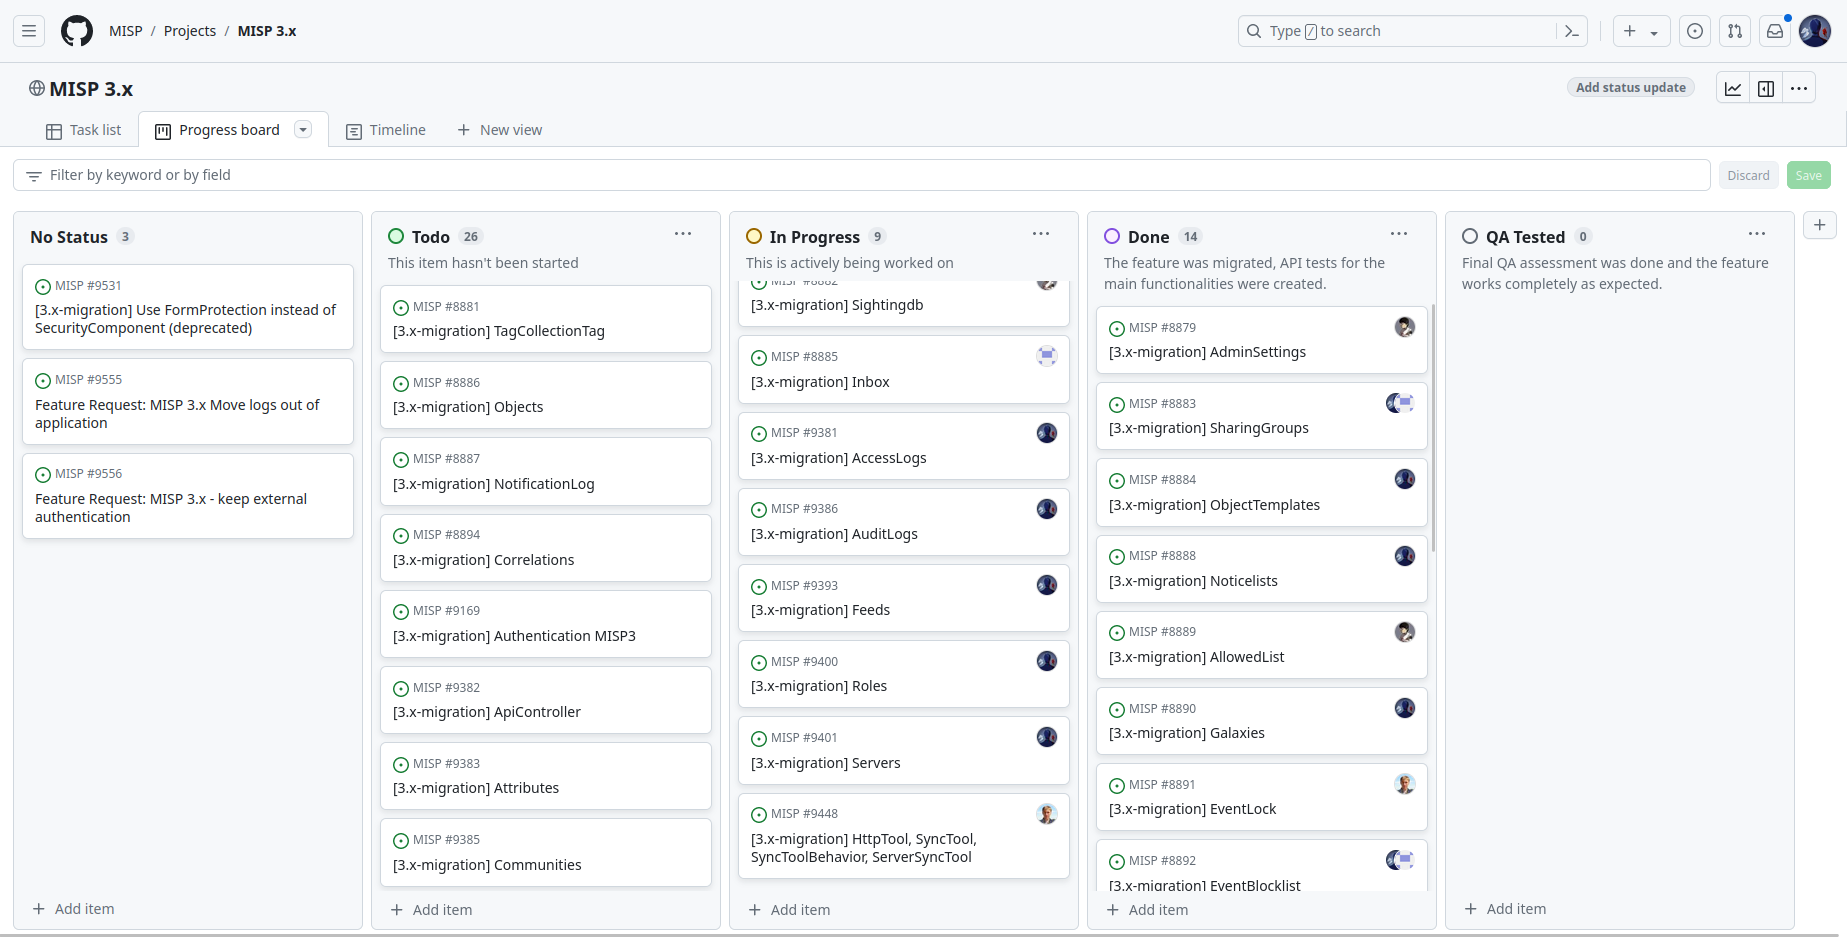
\includegraphics[scale=0.12]{misp3-project.png}
	\end{center}
	\begin{itemize}
		\item 26 Pull Requests (1 Open, 1 Draft)
		\item {\bf +105,165 lines of code added} and {\bf 20,992 lines of code removed}
	\end{itemize}
\end{frame}

\begin{frame}
        \frametitle{3.x - UI revamp}
	\begin{itemize}
	    \item {\bf Event View Page Redesign} - We are working on a complete overhaul of this page, with a focus on catering to multiple use-cases for different user-personas, enhancing responsiveness, integrating multiple charts, and emphasizing critical elements of MISP events. We’re also separating attributes and objects for clearer comprehension.
	    \item {\bf Navigation Menu Redesign} - We’re restructuring the navigation menu for better organization, incorporating intuitive groupings, icons, and support for mobile devices through a hamburger menu.
	    \item {\bf Bootstrap Upgrade} - Moving from Bootstrap 2 to Bootstrap 4 ensures a more modern and adaptable framework.
	\end{itemize}
\end{frame}

\begin{frame}
        \frametitle{3.x - UI revamp}
	\begin{itemize}
		\item {\bf Application-Wide Color Schemes} - We’re introducing support for customizable color schemes, including the much-requested dark mode.
		\item {\bf Settings and Diagnostics Page Redesign} - These sections will undergo a makeover to improve usability, accessibility and make them less overwhelming.
		\item {\bf Removal of Deprecated Features} - We aim to focus MISP’s functionality on core capabilities, we’re eliminating deprecated features that are no longer actively used or supported. This includes functionalities like Discussions or Threads, News, Scheduled Tasks, and Populate Event from Template.
	\end{itemize}
\end{frame}

\begin{frame}
        \frametitle{3.x - UI example}
	\begin{center}
		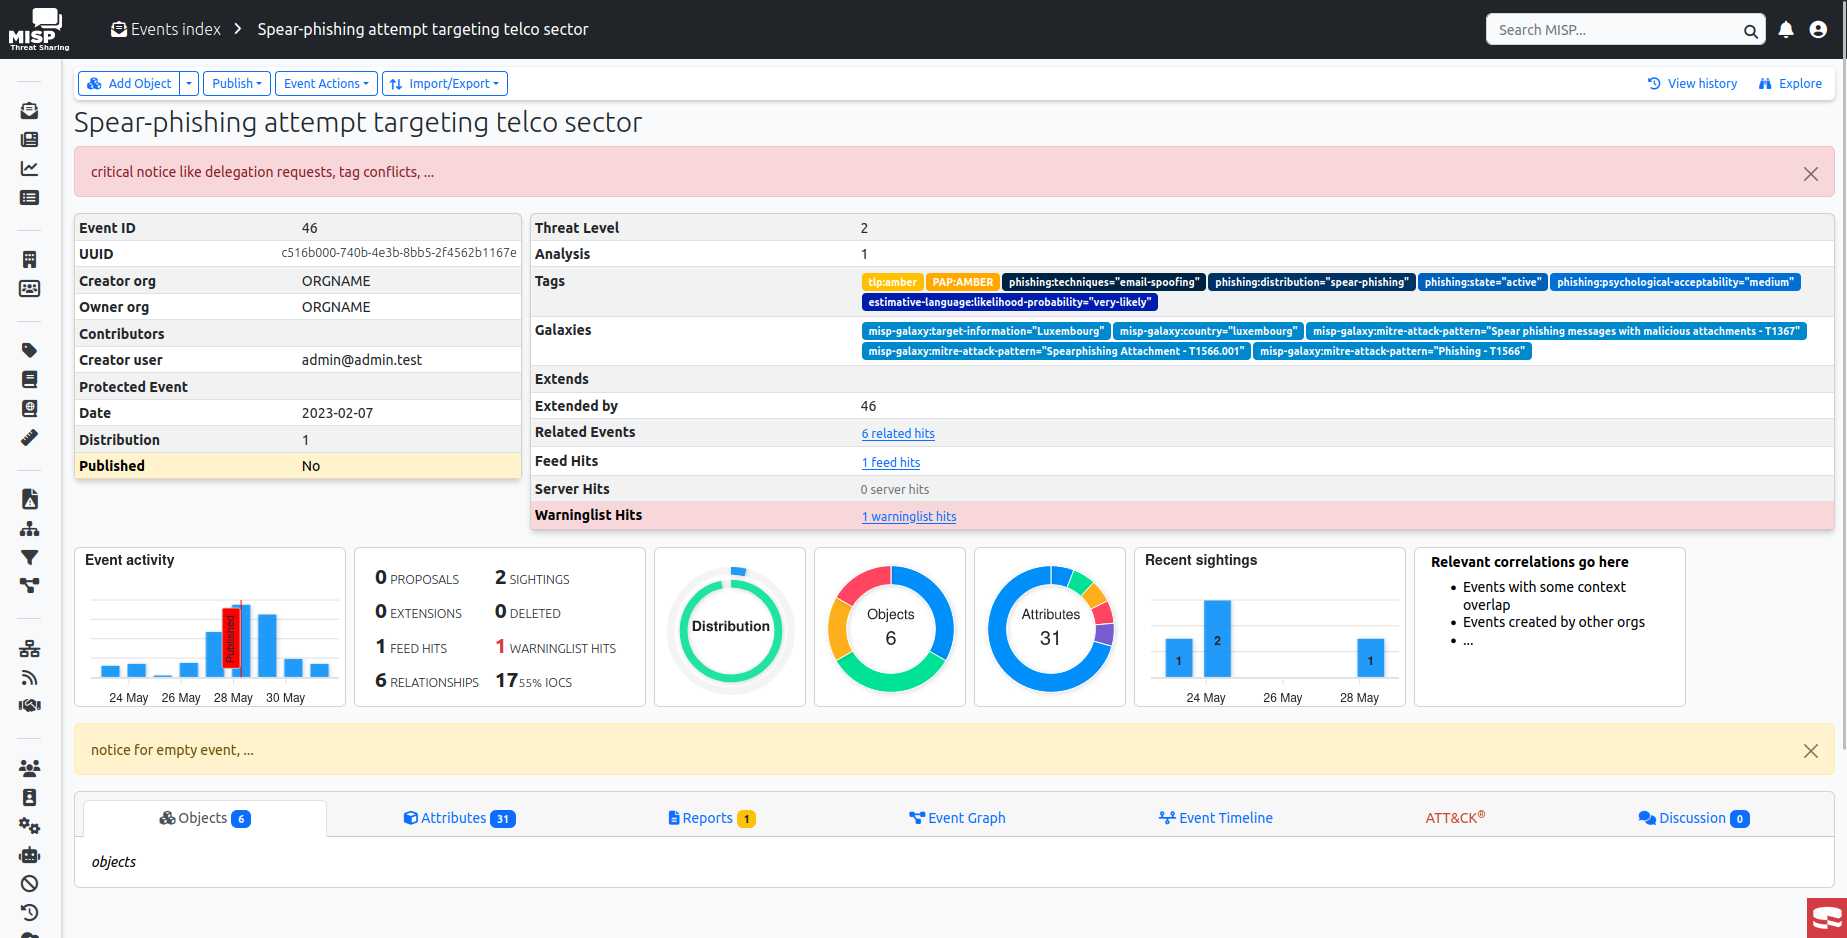
\includegraphics[scale=0.15]{misp3-ui.png}
	\end{center}
\end{frame}


\begin{frame}[fragile]
        \frametitle{3.x - Improved developer/deployment experience}
	\begin{itemize}
		\item Easy developer onboarding with dedicated readmes for development/testing.
		\item No more complex setup script, running docker development enviroment with just 3 commands:
	\end{itemize}
\begin{lstlisting}[basicstyle=\ttfamily\small, breaklines=true]
$ git clone -b 3.x git@github.com:MISP/MISP.git MISP3
$ cd MISP3
$ docker-compose -f docker-compose.yml -f docker-compose.dev.yml --env-file="./docker/.env.dev" up
\end{lstlisting}
\end{frame}

\begin{frame}
        \frametitle{3.x - Automatic checks/fixes via via pre-commit hooks}
	\begin{itemize}
		\item {\bf phpcbf}: Code style beautifying.
		\item {\bf phpcs}: Code style analysis PSR, naming conventions, etc.
		\item {\bf phpstan}: Automatic static code analysis unused variables/imports, forbidden functions, etc.
	\end{itemize}
\end{frame}

\begin{frame}[fragile]
	\frametitle{3.x - New test suite}
	\begin{itemize}
		\item Automatic API schema tests on requests/responses against OpenAPI spec.
		\item Code coverage.
		\item Testing sync and complex features mocking external http requests.
		\item Faster than previous PyMISP test suite.
		\item Reproducible, same tests are run by GitHub Actions on each PR.
		\item Easy to run, just one command:
	\end{itemize}
	\begin{lstlisting}[basicstyle=\ttfamily\small, breaklines=true,]
docker-compose -f docker-compose.yml -f docker-compose.dev.yml --env-file="./docker/.env.test" exec misp vendor/bin/phpunit
	\end{lstlisting}
\end{frame}

\begin{frame}
  \frametitle{MISP Airgap}
  \begin{itemize}
    \item MISP Airgap\footnote{\url{https://www.misp-project.org/2024/01/12/MISP-airgap.html/}} is a solution designed to \textbf{deploy MISP in air-gapped or isolated networks}.
    \item By leveraging the power of Linux containers (LXD), it ensures a secure, efficient, and manageable deployment of MISP instances.
    \item Furthermore, it enables users to frequently update their MISP instance in an environment cut off from the internet.
  \end{itemize}
\end{frame}

\begin{frame}
  \frametitle{To Sum It All Up...}
  \begin{itemize}
     \item The MISP \textbf{developer/contributor community} continues to grow and is very active.
     \item The main focus over the past months has been:
     \begin{itemize}
          \item Performance, security, and monitoring
          \item Improved deployment of MISP via the new misp-docker or misp-airgap
          \item Enhancing the documentation and supporting materials such as misp-playbooks
          \item Improving the MISP ecosystem, including misp-galaxy, misp-modules, and interconnectivity with new tools such as Flowintel
     \end{itemize}
     \item There is definitely no lack of new ideas and improvements. If you want to participate, it's easy to \textbf{get involved}.
\end{itemize}
\end{frame}

\begin{frame}
  \frametitle{Get in touch if you have any questions}
  \begin{itemize}
    \item Contact CIRCL
    \begin{itemize}
      \item info@circl.lu
      \item \url{https://social.circl.lu/@circl}
      \item \url{https://www.circl.lu/}
    \end{itemize}
    \item Contact MISPProject 
    \begin{itemize}
      \item \url{https://github.com/MISP}
      \item \url{https://gitter.im/MISP/MISP}
      \item \url{https://misp-community.org/@misp}
    \end{itemize}
    \item Cerebrate project
    \begin{itemize}
      \item \url{https://github.com/cerebrate-project}
      \item \url{https://github.com/cerebrate-project/cerebrate}
    \end{itemize}
  \end{itemize}
\end{frame}
